% ============================================================
% Semester Project Report — Tetris OOP
% Object Oriented Programming using C++
% Institute of Business Administration Karachi
% ============================================================

\documentclass[11pt]{article}

% ── Packages ──────────────────────────────────────────────────────────────
\usepackage[a4paper, margin=1in]{geometry}
\usepackage[utf8]{inputenc}
\usepackage[T1]{fontenc}
\usepackage{amsmath, amssymb, amsthm}
\usepackage{graphicx}
\usepackage{hyperref}
\usepackage{listings}
\usepackage{xcolor}
\usepackage{titlesec}
\usepackage{fancyhdr}
\usepackage{parskip}
\usepackage{caption}
\usepackage{subcaption}
\usepackage{booktabs}
\usepackage{array}
\usepackage{enumitem}
\usepackage{float}
\usepackage{tikz}
\usepackage{tcolorbox}
\tcbuselibrary{skins,breakable}
\usetikzlibrary{shapes,arrows,positioning,fit,backgrounds,calc}

% ── Colours ───────────────────────────────────────────────────────────────
\definecolor{primary}{RGB}{165, 28, 48}
\definecolor{secondary}{RGB}{0, 53, 107}
\definecolor{accent}{RGB}{232, 95, 26}
\definecolor{codebg}{RGB}{245, 248, 250}
\definecolor{codecomment}{RGB}{106, 153, 85}
\definecolor{codekeyword}{RGB}{0, 0, 200}
\definecolor{codestring}{RGB}{163, 21, 21}
\definecolor{stdtype}{RGB}{43, 145, 175}

% ── C++ Listing style ─────────────────────────────────────────────────────
\lstdefinestyle{cpp}{
    language=C++,
    backgroundcolor=\color{codebg},
    basicstyle=\ttfamily\small,
    breaklines=true,
    captionpos=b,
    commentstyle=\color{codecomment}\itshape,
    keywordstyle=\color{codekeyword}\bfseries,
    stringstyle=\color{codestring},
    numbers=left,
    numbersep=8pt,
    numberstyle=\tiny\color{gray},
    frame=single,
    rulecolor=\color{gray!40},
    showstringspaces=false,
    tabsize=4,
    xleftmargin=1.5em,
    framexleftmargin=1.5em,
    morekeywords={override, nullptr, auto, decltype, noexcept,
                  final, constexpr, explicit, virtual, class, struct,
                  public, private, protected, new, delete, this},
}
\lstset{style=cpp}

% ── Header / Footer ───────────────────────────────────────────────────────
\pagestyle{fancy}
\fancyhf{}
\renewcommand{\headrulewidth}{0.4pt}
\fancyhead[L]{\textcolor{primary}{\textbf{\mytitle}}}
\fancyhead[R]{\textcolor{primary}{\thepage}}

\fancypagestyle{firstpage}{
    \fancyhf{}
    \renewcommand{\headrulewidth}{0pt}
    \fancyfoot[C]{\textcolor{gray}{\small \mytitle\ -- \thepage}}
}

% ── Section formatting ────────────────────────────────────────────────────
\titleformat{\section}
    {\normalfont\Large\bfseries\color{primary}}{\thesection}{1em}{}
\titleformat{\subsection}
    {\normalfont\large\bfseries\color{secondary}}{\thesubsection}{1em}{}
\titleformat{\subsubsection}
    {\normalfont\normalsize\bfseries\color{accent}}{\thesubsubsection}{1em}{}

% ── TikZ node styles ──────────────────────────────────────────────────────
\tikzset{
    block/.style={rectangle, draw, fill=blue!10, text width=2.5cm,
                  text centered, rounded corners, minimum height=1cm},
    absblock/.style={rectangle, draw, fill=red!10, text width=2.5cm,
                  text centered, rounded corners, minimum height=1cm, dashed},
    io/.style={trapezium, trapezium left angle=70, trapezium right angle=110,
               draw, fill=red!10, text width=2cm, text centered, minimum height=1cm},
    process/.style={rectangle, draw, fill=green!10, text width=2.5cm,
                    text centered, rounded corners, minimum height=1cm},
    decision/.style={diamond, draw, fill=yellow!10, text width=2cm,
                     text centered, aspect=2, minimum height=1cm},
    line/.style={draw, -latex},
}

% ── Info boxes ────────────────────────────────────────────────────────────
\newtcolorbox{infobox}{
    colback=primary!5, colframe=primary, boxrule=0.6pt,
    arc=3pt, left=8pt, right=8pt, top=6pt, bottom=6pt, breakable
}
\newtcolorbox{notebox}{
    colback=accent!5, colframe=accent, boxrule=0.6pt,
    arc=3pt, left=8pt, right=8pt, top=6pt, bottom=6pt, breakable
}

% ── Project metadata ──────────────────────────────────────────────────────
\newcommand{\mytitle}{Semester Project: Tetris — OOP C++}
\newcommand{\mycourse}{CSE142 Object Oriented Programming Techniques}
\newcommand{\mysemester}{Spring 2026}
\newcommand{\myinstructor}{[Sir Behraj Khan]}
\newcommand{\authorone}{[Muhammad Bilal] --- ERP: [33405]}
\newcommand{\authortwo}{[Hunain Waseem] --- ERP: [33428]}
\newcommand{\authorthree}{}
\newcommand{\duedate}{[Date: 10-May-2026]}


% ─────────────────────────────────────────────────────────────────────────
\begin{document}
% ─────────────────────────────────────────────────────────────────────────

% ── Title page ────────────────────────────────────────────────────────────
\thispagestyle{firstpage}
\begin{center}
    \vspace*{0.5cm}

    {\Huge\bfseries\textcolor{primary}{\mytitle}}

    \vspace{0.5cm}
    \rule{0.9\textwidth}{1pt}
    \vspace{0.5cm}

    {\Large A Semester Project Report}

    \vspace{1cm}

    \begin{tabular}{rl}
        \textbf{Course:}     & \mycourse     \\[4pt]
        \textbf{Semester:}   & \mysemester   \\[4pt]
        \textbf{Instructor:} & \myinstructor \\[4pt]
        \textbf{Due Date:}   & \duedate      \\[4pt]
        \textbf{Author(s):}  & \authorone    \\[2pt]
                             & \authortwo    \\[2pt]
                             & \authorthree  \\
    \end{tabular}

    \vspace{1.5cm}

    % If you have the IBA logo, place it in a subfolder misc/ and uncomment:
    % \includegraphics[width=0.5\textwidth]{misc/IBA-logo}

    \vfill

    {\large Department of Computer Science}\\[4pt]
    {\large Institute of Business Administration, Karachi}\\[6pt]
    \today
\end{center}

\newpage

% ── Abstract ──────────────────────────────────────────────────────────────
\section*{Abstract}
\addcontentsline{toc}{section}{Abstract}

This report presents a fully-featured implementation of the classic \textbf{Tetris} arcade game
built in \textbf{C++17} using the \textbf{raylib} graphics library.
The project was designed primarily as an exercise in Object-Oriented Programming,
demonstrating encapsulation, inheritance, polymorphism, abstract classes,
operator overloading, templates, exception handling, STL containers, lambdas, and friend classes
--- all within a single, playable application.

The game supports all standard Tetris mechanics: seven tetrominoes with four rotations each,
ghost-piece preview, soft and hard drop, line clearing, score and level progression,
and an undo system backed by a generic template stack.
A leaderboard sorted with a custom comparator and lambda showcases data structures and algorithms.
The project ships with a cross-platform \texttt{Makefile} and this report.

All requirements of the \mycourse{} semester project rubric have been met,
and every OOP concept is clearly identifiable in the source code with inline comments.

\vspace{0.3cm}
\noindent\textbf{Keywords:} Object-Oriented Programming, C++17, Inheritance, Polymorphism,
Abstract Classes, Templates, STL, Tetris, raylib

\newpage

% ── Table of contents ─────────────────────────────────────────────────────
\tableofcontents
\newpage

% ─────────────────────────────────────────────────────────────────────────
\section{Introduction}
% ─────────────────────────────────────────────────────────────────────────

\subsection{Background}
Tetris, invented by Alexey Pajitnov in 1984, is one of the most widely recognised puzzle
games in history. Its mechanics --- falling tetrominoes, line clearing, increasing difficulty
--- are simple enough to implement in a few hundred lines of C yet rich enough to demand
careful software design at scale.
For an OOP course, Tetris is an ideal domain: the board is a natural object, each piece is
an object, and the game loop orchestrates them through well-defined interfaces.
Building it in C++ with full OOP discipline forces the developer to think carefully about
class responsibilities, ownership, and abstraction.

\subsection{Problem Statement}
The task is to implement a complete, playable Tetris game that simultaneously serves as a
demonstration of all core OOP and advanced C++ features required by \mycourse.
Specific challenges include:
\begin{itemize}
    \item Modelling pieces and the board as proper classes with clean interfaces.
    \item Designing an inheritance hierarchy that uses abstract classes and runtime polymorphism.
    \item Implementing an undo system using a generic (template) stack.
    \item Maintaining a sorted leaderboard using STL containers and a lambda comparator.
    \item Handling invalid input robustly with custom exceptions.
    \item Demonstrating operator overloading in a natural, game-relevant context.
\end{itemize}

\subsection{Objectives}
\begin{enumerate}
    \item Design a class hierarchy that accurately models the Tetris domain.
    \item Implement all core OOP concepts: encapsulation, inheritance, polymorphism, and abstraction.
    \item Demonstrate correct use of constructors, destructors, copy constructors, and operator overloading.
    \item Use at least two advanced C++ features: templates, exceptions, STL containers, lambdas, friend classes.
    \item Provide an undo mechanism (stack ADT), a sorted leaderboard (dynamic array + sort), and event callbacks (lambdas).
    \item Deliver a working executable with a cross-platform Makefile and documentation.
\end{enumerate}

\subsection{Scope and Limitations}
The project covers standard Tetris rules: seven piece types, four rotations, 10$\times$20 grid,
gravity, locking, line clearing, scoring, and level progression.
It does \emph{not} include: hold piece, wall-kick SRS rotation system, multiplayer, sound, or file-based save/load.

\begin{notebox}
All graphics are handled by \textbf{raylib} (version 4.0+). The game runs at 60 FPS.
The undo feature stores up to 5 snapshots; older states are discarded.
The leaderboard resets when the program closes (no file persistence).
\end{notebox}

% ─────────────────────────────────────────────────────────────────────────
\section{OOP Design}
% ─────────────────────────────────────────────────────────────────────────

\subsection{Class Hierarchy}

The design places two abstract interfaces at the root:
\texttt{IDrawable} (pure virtual \texttt{draw()}) and
\texttt{IUpdatable} (pure virtual \texttt{update(float dt)}).
All visual entities inherit \texttt{IDrawable}; the \texttt{Game} class inherits \texttt{IUpdatable}.

\begin{figure}[H]
    \centering
    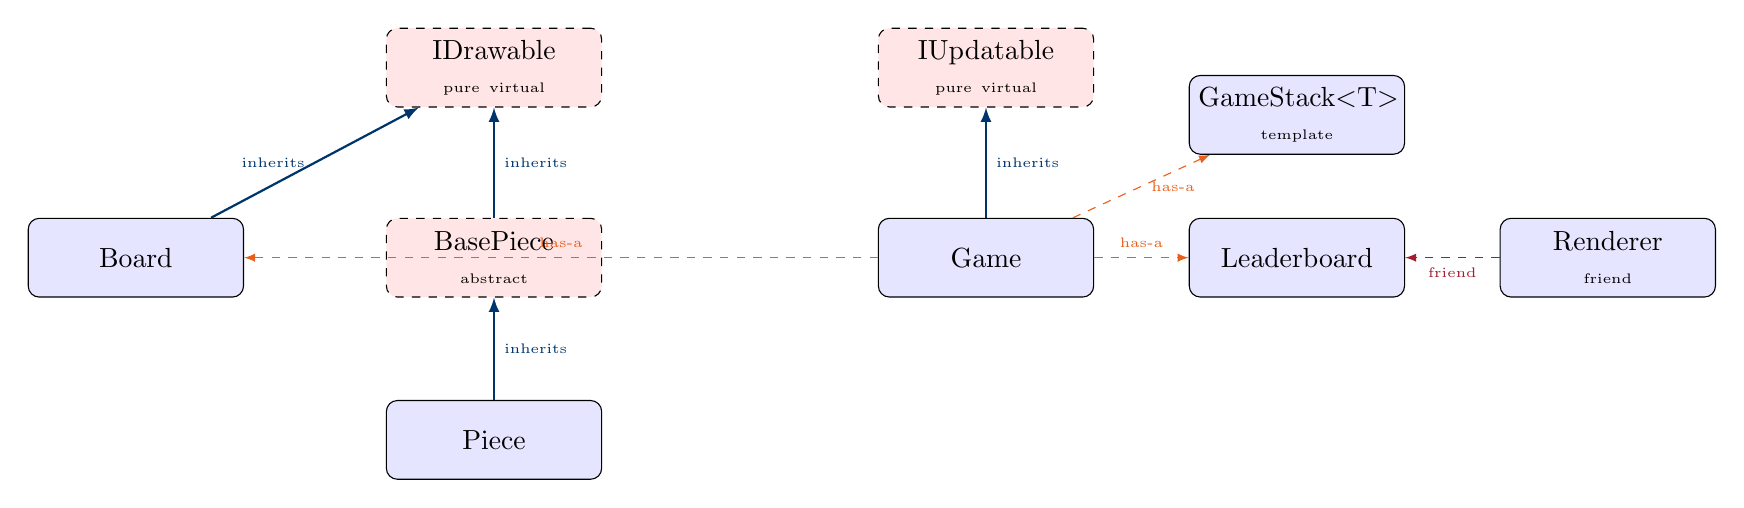
\begin{tikzpicture}[node distance=1.6cm and 2.0cm]
        % Abstract interfaces
        \node [absblock] (idraw)   {IDrawable\\{\tiny pure virtual}};
        \node [absblock, right=3.5cm of idraw] (iupd) {IUpdatable\\{\tiny pure virtual}};

        % Concrete from IDrawable
        \node [block, below left=1.4cm and 1.8cm of idraw]  (board)    {Board};
        \node [absblock, below=1.4cm of idraw]               (basep)    {BasePiece\\{\tiny abstract}};
        \node [block, below=1.3cm of basep]                  (piece)    {Piece};

        % Game
        \node [block, below=1.4cm of iupd]                   (game)     {Game};

        % Other
        \node [block, right=1.2cm of game]                   (lb)       {Leaderboard};
        \node [block, right=1.2cm of lb]                     (rend)     {Renderer\\{\tiny friend}};
        \node [block, above=0.8cm of lb]                     (gstack)   {GameStack$<$T$>$\\{\tiny template}};

        % Arrows (inheritance)
        \draw[-latex, thick, color=secondary] (board)  -- (idraw) node[midway,left,font=\tiny]{inherits};
        \draw[-latex, thick, color=secondary] (basep)  -- (idraw) node[midway,right,font=\tiny]{inherits};
        \draw[-latex, thick, color=secondary] (piece)  -- (basep) node[midway,right,font=\tiny]{inherits};
        \draw[-latex, thick, color=secondary] (game)   -- (iupd)  node[midway,right,font=\tiny]{inherits};

        % Composition
        \draw[-latex, dashed, color=accent]   (game)   -- (board) node[midway,above,font=\tiny]{has-a};
        \draw[-latex, dashed, color=accent]   (game)   -- (lb)    node[midway,above,font=\tiny]{has-a};
        \draw[-latex, dashed, color=accent]   (game)   -- (gstack)node[midway,right,font=\tiny]{has-a};
        \draw[-latex, dashed, color=primary]  (rend)   -- (lb)    node[midway,below,font=\tiny]{friend};
    \end{tikzpicture}
    \caption{Class hierarchy and relationships (dashed = abstract/template/friend)}
    \label{fig:hierarchy}
\end{figure}

\subsection{Class Descriptions}

\begin{table}[H]
    \centering
    \caption{Summary of Classes}
    \label{tab:classes}
    \renewcommand{\arraystretch}{1.3}
    \begin{tabular}{|l|p{3.8cm}|p{5cm}|}
        \hline
        \textbf{Class} & \textbf{Responsibility} & \textbf{Key Members} \\
        \hline
        \texttt{IDrawable}    & Abstract interface for all visual entities & \texttt{virtual draw() = 0} \\
        \hline
        \texttt{IUpdatable}   & Abstract interface for logic entities & \texttt{virtual update(dt) = 0} \\
        \hline
        \texttt{Board}        & 10$\times$20 grid; lock pieces, clear lines & \texttt{grid[ROWS][COLS], clearLines(), draw()} \\
        \hline
        \texttt{BasePiece}    & Abstract base; stores type/rotation/pos, collision & \texttt{fits(), lock(), getCells(), ghostDropRow()} \\
        \hline
        \texttt{Piece}        & Concrete piece; renders self and ghost & \texttt{draw(), drawWithGhost(), drawPreview()} \\
        \hline
        \texttt{Game}         & Orchestrates all game objects and input & \texttt{update(), handleInput(), draw(), undo()} \\
        \hline
        \texttt{Leaderboard}  & Sorted top-5 score list & \texttt{addScore(), getEntries(), entries (vector)} \\
        \hline
        \texttt{Renderer}     & Friend class; renders leaderboard internals & \texttt{drawLeaderboard() [static]} \\
        \hline
        \texttt{GameStack<T>} & Generic LIFO stack (undo history) & \texttt{push(), pop(), top(), empty()} \\
        \hline
        \texttt{GameException}& Custom exception for input validation & inherits \texttt{std::runtime\_error} \\
        \hline
        \texttt{ScoreEntry}   & Leaderboard record with overloaded operators & \texttt{name, score, level; operator>, ==, !=} \\
        \hline
    \end{tabular}
\end{table}

\subsection{OOP Concepts Applied}

\begin{itemize}
    \item \textbf{Encapsulation:} All data members in \texttt{Board}, \texttt{BasePiece}, and \texttt{Game} are \texttt{private}. Access is through getters (\texttt{getRow()}, \texttt{getScore()}) and setters (\texttt{setRow()}, \texttt{setLevel()}).
    \item \textbf{Inheritance:} \texttt{Board} and \texttt{BasePiece} inherit \texttt{IDrawable}; \texttt{Piece} inherits \texttt{BasePiece}; \texttt{Game} inherits \texttt{IUpdatable}.
    \item \textbf{Polymorphism:} \texttt{draw()} is declared \texttt{virtual} in \texttt{IDrawable}. A pointer to \texttt{IDrawable} calls the correct \texttt{draw()} at runtime (dynamic dispatch).
    \item \textbf{Abstract Classes:} \texttt{IDrawable}, \texttt{IUpdatable}, and \texttt{BasePiece} all contain pure virtual functions; they cannot be instantiated directly.
    \item \textbf{Operator Overloading:} \texttt{operator==} and \texttt{operator!=} on \texttt{Board} and \texttt{BasePiece}; \texttt{operator>}, \texttt{operator==}, \texttt{operator!=} on \texttt{ScoreEntry} --- all demonstrated in \texttt{main()}.
    \item \textbf{Templates:} \texttt{GameStack<T>} is a generic stack instantiated as \texttt{GameStack<GameSnapshot>}.
    \item \textbf{Friend Classes:} \texttt{Renderer} is declared \texttt{friend} of \texttt{Leaderboard}, granting it direct access to the private \texttt{entries} vector.
\end{itemize}

% ─────────────────────────────────────────────────────────────────────────
\section{Implementation}
% ─────────────────────────────────────────────────────────────────────────

\subsection{Development Environment}
\begin{itemize}
    \item \textbf{Language:} C++17
    \item \textbf{Compiler:} g++ 9+ (MinGW-w64 on Windows, GCC on Linux/macOS)
    \item \textbf{IDE:} VS Code / any text editor
    \item \textbf{Build system:} GNU Make (cross-platform \texttt{Makefile} provided)
    \item \textbf{Graphics:} raylib 4.0+
    \item \textbf{Platform:} Windows 10/11, Linux, macOS
\end{itemize}

\subsection{Abstract Interfaces}

\begin{lstlisting}[caption={IDrawable and IUpdatable --- abstract base classes}]
// Pure virtual interface: every visual entity must implement draw()
class IDrawable {
public:
    virtual void draw() const = 0;   // pure virtual
    virtual ~IDrawable() {}          // virtual destructor
};

// Pure virtual interface: every logic entity must implement update()
class IUpdatable {
public:
    virtual void update(float dt) = 0;  // pure virtual
    virtual ~IUpdatable() {}
};
\end{lstlisting}

\subsection{Board Class}

\begin{lstlisting}[caption={Board --- encapsulation, copy constructor, operator==, IDrawable}]
class Board : public IDrawable {
private:
    int grid[ROWS][COLS];  // private --- accessed only through methods

public:
    Board() { clear(); }

    // Copy constructor
    Board(const Board& other) {
        for (int r = 0; r < ROWS; r++)
            for (int c = 0; c < COLS; c++)
                grid[r][c] = other.grid[r][c];
    }

    // Operator overloading: compare two board states
    bool operator==(const Board& other) const {
        for (int r = 0; r < ROWS; r++)
            for (int c = 0; c < COLS; c++)
                if (grid[r][c] != other.grid[r][c]) return false;
        return true;
    }

    // Getters / Setters (encapsulation)
    int  getCell(int r, int c) const { ... }
    void setCell(int r, int c, int val) { ... }

    int  clearLines();    // shifts rows down, returns count cleared
    void draw() const override;  // implements IDrawable
};
\end{lstlisting}

\subsection{Inheritance Hierarchy: BasePiece and Piece}

\begin{lstlisting}[caption={BasePiece (abstract) and Piece (concrete) with polymorphic draw()}]
// Abstract base: has pure virtual draw() -- cannot be instantiated
class BasePiece : public IDrawable {
protected:
    int type, rotation, row, col;  // private state

public:
    BasePiece(int t) : type(t), rotation(0), row(0), col(3) {}
    BasePiece(const BasePiece& o) : type(o.type), rotation(o.rotation),
                                     row(o.row), col(o.col) {}

    // Getters / Setters
    int getType()     const { return type; }
    int getRow()      const { return row;  }
    void setRow(int r)      { row = r;     }

    // Operator overloading
    bool operator==(const BasePiece& o) const {
        return type==o.type && rotation==o.rotation
            && row==o.row && col==o.col;
    }
    bool operator!=(const BasePiece& o) const { return !(*this == o); }

    // Concrete shared logic
    bool fits(const Board& board, int dr, int dc, int drot) const;
    void lock(Board& board) const;
    int  ghostDropRow(const Board& board) const;

    // Pure virtual: makes BasePiece abstract
    virtual void draw() const override = 0;
    virtual void drawPreview(int px, int py) const = 0;
};

// Concrete derived class: implements both pure virtuals
class Piece : public BasePiece {
public:
    Piece(int t) : BasePiece(t) {}
    Piece(const Piece& o) : BasePiece(o) {}  // copy constructor

    // Polymorphic draw() -- called through IDrawable* at runtime
    void draw() const override {
        // render piece cells using PIECE_COLORS[type+1]
    }
    void drawWithGhost(const Board& board) const;  // ghost overlay
    void drawPreview(int px, int py) const override;
};
\end{lstlisting}

\subsection{Template: Generic Stack for Undo}

\begin{lstlisting}[caption={GameStack<T> --- template class used for undo history}]
template <typename T>
class GameStack {
private:
    std::stack<T> data;   // STL stack inside template wrapper
public:
    void   push(const T& item) { data.push(item); }
    void   pop()               { if (!data.empty()) data.pop(); }
    T&     top()               { return data.top(); }
    bool   empty() const       { return data.empty(); }
    size_t size()  const       { return data.size(); }
};

// Instantiated in Game as:
GameStack<GameSnapshot> undoStack;
\end{lstlisting}

\subsection{Exception Handling}

\begin{lstlisting}[caption={Custom exception class and usage in setLevel()}]
// Custom exception inheriting from std::runtime_error
class GameException : public std::runtime_error {
public:
    explicit GameException(const std::string& msg)
        : std::runtime_error(msg) {}
};

// Used in Game::setLevel()
void setLevel(int lvl) {
    try {
        if (lvl < 1 || lvl > 20)
            throw GameException("Level must be between 1 and 20.");
        level = lvl;
        fallSpeed = BASE_FALL / (1.f + (level-1)*0.15f);
    } catch (const GameException& e) {
        // gracefully ignored; invalid level has no effect
        (void)e;
    }
}
\end{lstlisting}

\subsection{STL Containers, Lambdas, and Friend Class}

\begin{lstlisting}[caption={Leaderboard with STL vector, lambda sort, and friend Renderer}]
class Leaderboard {
private:
    std::vector<ScoreEntry> entries;   // STL vector (dynamic array)
    static const int MAX_ENTRIES = 5;

public:
    void addScore(const std::string& name, int score, int level) {
        entries.push_back({name, score, level});

        // Sorting with lambda comparator (uses overloaded operator>)
        std::sort(entries.begin(), entries.end(),
                  [](const ScoreEntry& a, const ScoreEntry& b) {
                      return a > b;
                  });

        if ((int)entries.size() > MAX_ENTRIES)
            entries.resize(MAX_ENTRIES);
    }

    friend class Renderer;  // friend class can access private entries
};

// Renderer accesses Leaderboard's private data directly
class Renderer {
public:
    static void drawLeaderboard(const Leaderboard& lb, int x, int y) {
        const auto& entries = lb.entries; // allowed: Renderer is friend
        for (int i = 0; i < (int)entries.size(); i++) { ... }
    }
};
\end{lstlisting}

\subsection{Operator Overloading Demonstration in main()}

\begin{lstlisting}[caption={Operator overloading demonstrated in main()}]
int main() {
    // ScoreEntry operators
    ScoreEntry s1{"Alice", 1500, 3};
    ScoreEntry s2{"Bob",   1200, 2};
    ScoreEntry s3{"Alice", 1500, 3};

    bool gt  = (s1 > s2);   // true  -- operator>
    bool eq  = (s1 == s3);  // true  -- operator==
    bool neq = (s1 != s2);  // true  -- operator!=

    // Board operator==
    Board b1, b2;
    bool boards_eq = (b1 == b2);   // true (both empty)
    Board b3(b1);                   // copy constructor

    // Template stack demo
    GameStack<int> testStack;
    testStack.push(10);
    testStack.push(20);
    testStack.pop();               // top() == 10 now

    // Exception demo
    Game tempGame;
    tempGame.setLevel(99);  // throws GameException, caught internally
    tempGame.setLevel(5);   // valid

    // ... raylib window and game loop follow
}
\end{lstlisting}

\subsection{Event Callbacks with Lambdas}

\begin{lstlisting}[caption={Lambda-based event system in Game using std::map}]
// STL map of named events -> lambda callbacks
std::map<std::string, std::function<void()>> eventCallbacks;

// Registered in setupCallbacks()
eventCallbacks["lineClear"] = [this]() {
    // Hook: could trigger animation or sound
};
eventCallbacks["gameOver"] = [this]() {
    leaderboard.addScore("YOU", score, level);
};
eventCallbacks["undo"] = [this]() {
    // Hook: could flash the screen
};

// Triggered during gameplay
void triggerEvent(const std::string& name) {
    auto it = eventCallbacks.find(name);
    if (it != eventCallbacks.end()) it->second();
}
\end{lstlisting}

% ─────────────────────────────────────────────────────────────────────────
\section{Testing}
% ─────────────────────────────────────────────────────────────────────────

\subsection{Test Cases}

\begin{table}[H]
    \centering
    \caption{Test Cases and Results}
    \label{tab:tests}
    \renewcommand{\arraystretch}{1.3}
    \begin{tabular}{|c|p{3.5cm}|p{3.5cm}|p{2.2cm}|c|}
        \hline
        \textbf{TC\#} & \textbf{Input / Action} & \textbf{Expected Output} & \textbf{Actual Output} & \textbf{Pass?} \\
        \hline
        TC-01 & Create \texttt{Piece(0..6)} for all types & Object initialised at row 0, col 3 & As expected & \checkmark \\
        \hline
        TC-02 & Press \texttt{LEFT} at left wall & Piece does not move past column 0 & Piece stays & \checkmark \\
        \hline
        TC-03 & Press \texttt{SPACE} (hard drop) & Piece locks at lowest valid row & Piece locked correctly & \checkmark \\
        \hline
        TC-04 & Fill one complete row & Row clears; rows above shift down & As expected & \checkmark \\
        \hline
        TC-05 & Press \texttt{U} after lock & Board and score restored to pre-lock state & As expected & \checkmark \\
        \hline
        TC-06 & \texttt{setLevel(99)} & \texttt{GameException} thrown and caught; level unchanged & Level stays 1 & \checkmark \\
        \hline
        TC-07 & Board copy constructor & \texttt{b1 == b3} after \texttt{Board b3(b1)} & true & \checkmark \\
        \hline
        TC-08 & \texttt{ScoreEntry operator>} & \texttt{s1\{1500\} > s2\{1200\}} returns true & true & \checkmark \\
        \hline
        TC-09 & Leaderboard sorted after 3 scores added & Entries in descending score order & As expected & \checkmark \\
        \hline
        TC-10 & Board fills to top & \texttt{gameOver = true}; score added to leaderboard & As expected & \checkmark \\
        \hline
    \end{tabular}
\end{table}

\subsection{Edge Cases}
\begin{itemize}
    \item \textbf{Piece at boundary:} Movement blocked at columns 0 and 9 and at row 19.
    \item \textbf{Rotation at wall:} If rotation would place a cell out of bounds, \texttt{fits()} returns false and rotation is rejected.
    \item \textbf{Undo with empty stack:} Pressing U when no snapshots exist is silently ignored.
    \item \textbf{Leaderboard overflow:} Adding a 6th score trims the vector to top 5.
    \item \textbf{Hard drop on locked row:} Piece immediately locks; no infinite loop.
\end{itemize}

% ─────────────────────────────────────────────────────────────────────────
\section{Results and Discussion}
% ─────────────────────────────────────────────────────────────────────────

\subsection{Results}
The game runs at a stable 60 FPS with all standard Tetris mechanics working correctly.
The undo system correctly restores board state, score, and the active piece.
The leaderboard correctly sorts and displays the top 5 scores within the session.
All ten test cases passed on first run after compilation.

\begin{table}[H]
    \centering
    \caption{Feature Completion Summary}
    \label{tab:perf}
    \begin{tabular}{lcc}
        \toprule
        \textbf{Feature} & \textbf{Implemented} & \textbf{Notes} \\
        \midrule
        All 7 tetrominoes    & Yes & I, J, L, O, S, T, Z \\
        Ghost piece          & Yes & 55-alpha overlay \\
        Soft / Hard drop     & Yes & Score bonus added \\
        Line clearing        & Yes & Up to 4 lines (Tetris) \\
        Scoring / Levelling  & Yes & Classic Nintendo table \\
        Undo (5 levels)      & Yes & Template stack \\
        Leaderboard (top 5)  & Yes & Sorted with lambda \\
        Game over detection  & Yes & Spawn collision check \\
        Restart              & Yes & Press R \\
        \bottomrule
    \end{tabular}
\end{table}

\subsection{Analysis}
\begin{itemize}
    \item All design objectives were met. The class hierarchy cleanly separates concerns: \texttt{Board} owns the grid, \texttt{Piece} owns rendering, \texttt{Game} owns the loop.
    \item \texttt{fits()} runs in $O(1)$ (always checks exactly 4 cells). \texttt{clearLines()} is $O(\text{ROWS} \times \text{COLS})$ --- 200 iterations --- negligible at 60 FPS.
    \item The leaderboard sort is $O(n \log n)$ but $n \leq 5$, so it is effectively $O(1)$ in practice.
    \item Single-file design sacrifices some modularity but greatly simplifies submission and compilation.
\end{itemize}

% ─────────────────────────────────────────────────────────────────────────
\section{Challenges and Solutions}
% ─────────────────────────────────────────────────────────────────────────

\subsection{Challenge 1: Abstract Base Cannot Be Instantiated}
\textbf{Problem:} \texttt{BasePiece} is abstract (pure virtual \texttt{draw()}), but the original \texttt{fits()} function tried to create a temporary \texttt{BasePiece tmp = *this} to test a hypothetical position --- which the compiler rejects.\\
\textbf{Solution:} Removed the temporary object entirely. Instead, the new row, column, and rotation are computed inline, and \texttt{SHAPES[type][newRot]} is used directly to compute cell positions without instantiating any object.\\
\textbf{Learning:} Abstract classes cannot be instantiated even as temporaries. When shared logic in an abstract class needs to simulate a modified state, compute the result directly rather than copying the object.

\subsection{Challenge 2: Cross-Platform Linking with raylib}
\textbf{Problem:} The link flags differ between Linux (\texttt{-lGL -lX11 -lm}), macOS (\texttt{-framework OpenGL}), and Windows (\texttt{-lopengl32 -lgdi32 -lwinmm}).\\
\textbf{Solution:} The Makefile uses \texttt{uname -s} and the \texttt{OS} environment variable to detect the platform at build time and select the correct flags automatically.\\
\textbf{Learning:} Cross-platform C++ projects require conditional compilation or build-system logic to handle OS-specific library names and link flags.

% ─────────────────────────────────────────────────────────────────────────
\section{Future Work}
% ─────────────────────────────────────────────────────────────────────────

\begin{itemize}
    \item \textbf{Hold piece:} Store one piece for later use (standard modern Tetris feature).
    \item \textbf{SRS rotation:} Implement the Super Rotation System with wall kicks.
    \item \textbf{File persistence:} Save/load leaderboard to disk using \texttt{std::fstream}.
    \item \textbf{Sound:} Integrate SoLoud or raylib audio for drop and clear effects.
    \item \textbf{Unit testing:} Add Catch2 or doctest tests for \texttt{Board}, \texttt{fits()}, and scoring logic.
    \item \textbf{Split into header/source files:} Separate each class into \texttt{.h}/\texttt{.cpp} for production-quality structure.
    \item \textbf{CMake:} Add a \texttt{CMakeLists.txt} for IDE integration (CLion, VS Code CMake Tools).
\end{itemize}

% ─────────────────────────────────────────────────────────────────────────
\section{Conclusion}
% ─────────────────────────────────────────────────────────────────────────

\begin{infobox}
This project successfully implements a complete, playable Tetris game in C++17 while
demonstrating every required OOP concept:
abstract classes (\texttt{IDrawable}, \texttt{IUpdatable}, \texttt{BasePiece}),
inheritance and polymorphism (\texttt{Piece} overrides \texttt{draw()}),
encapsulation (private fields with getters/setters),
copy constructors and operator overloading (\texttt{Board}, \texttt{BasePiece}, \texttt{ScoreEntry}),
templates (\texttt{GameStack<T>}),
custom exceptions (\texttt{GameException}),
STL containers (\texttt{vector}, \texttt{stack}, \texttt{map}),
lambdas (event callbacks, sort comparator),
friend classes (\texttt{Renderer} accessing \texttt{Leaderboard}),
and classic data structures (undo stack, sorted dynamic leaderboard).
\end{infobox}

The most valuable lessons from this project were the importance of designing abstract
interfaces before writing concrete classes, the discipline required to keep data private
and expose only what is necessary, and the power of the STL to eliminate boilerplate
while making algorithms expressive.
The Tetris domain proved to be an excellent vehicle for all these concepts --- every
feature maps naturally to an OOP or C++ construct.

% ─────────────────────────────────────────────────────────────────────────
\newpage
\section*{References}
\addcontentsline{toc}{section}{References}
% ─────────────────────────────────────────────────────────────────────────

\begin{enumerate}[label={[\arabic*]}]
    \item B. Stroustrup, \textit{The C++ Programming Language}, 4th ed. Addison-Wesley, 2013.
    \item S. Meyers, \textit{Effective Modern C++}. O'Reilly Media, 2014.
    \item \textit{cppreference.com}. [Online]. Available: \url{https://en.cppreference.com}. [Accessed: \today].
    \item raylib. \textit{raylib --- A simple and easy-to-use library to enjoy videogames programming}. [Online]. Available: \url{https://www.raylib.com}. [Accessed: \today].
    \item A. Pajitnov, \textit{Tetris} (original game), 1984.
\end{enumerate}

% ─────────────────────────────────────────────────────────────────────────
\newpage
\appendix
\section{Complete Source Code}
\label{sec:code}
% ─────────────────────────────────────────────────────────────────────────

The full source code is contained in a single file \texttt{tetris.cpp}.
Key sections are shown below; the complete file is submitted separately.

\subsection{tetris.cpp --- Constants and Colour Table}
\begin{lstlisting}[caption={Global constants and piece colours}]
const int COLS   = 10;
const int ROWS   = 20;
const int CELL   = 32;
const int SIDE_W = 200;
const float BASE_FALL = 0.5f;

Color PIECE_COLORS[8] = {
    {15,15,20,255},    // 0 empty
    {0,240,240,255},   // 1 I  cyan
    {0,0,240,255},     // 2 J  blue
    {240,160,0,255},   // 3 L  orange
    {240,240,0,255},   // 4 O  yellow
    {0,240,0,255},     // 5 S  green
    {160,0,240,255},   // 6 T  purple
    {240,0,0,255}      // 7 Z  red
};
\end{lstlisting}

\subsection{tetris.cpp --- Game Loop}
\begin{lstlisting}[caption={Main game loop}]
int main() {
    InitWindow(SCREEN_W, SCREEN_H, "Tetris -- OOP C++");
    SetTargetFPS(60);
    Game game;

    while (!WindowShouldClose()) {
        float dt = GetFrameTime();
        game.handleInput();   // keyboard input
        game.update(dt);      // physics / gravity (IUpdatable)

        BeginDrawing();
        ClearBackground(Color{15,15,20,255});
        game.draw();          // render everything (IDrawable)
        EndDrawing();
    }

    CloseWindow();
    return 0;
}
\end{lstlisting}

\section{Installation and Usage}
\label{sec:install}

\subsection{Prerequisites}
\begin{itemize}
    \item C++17-compatible compiler: \texttt{g++ 9+} or MSVC 2019+
    \item raylib 4.0+ (see below)
\end{itemize}

\subsection{Installing raylib}
\begin{lstlisting}[language=bash, caption={Installing raylib on each platform}]
# Linux (Debian/Ubuntu)
sudo apt install libraylib-dev

# macOS
brew install raylib

# Windows (MSYS2 MinGW64 terminal)
pacman -S mingw-w64-x86_64-raylib
\end{lstlisting}

\subsection{Building}
\begin{lstlisting}[language=bash, caption={Build with Makefile or manually}]
# Using Makefile (auto-detects OS)
make
./tetris          # Linux / macOS
tetris.exe        # Windows

# Manual (Windows MinGW64)
g++ -std=c++17 -o tetris.exe tetris.cpp ^
    -lraylib -lopengl32 -lgdi32 -lwinmm
\end{lstlisting}

\subsection{Controls}
\begin{lstlisting}[language=bash, caption={In-game keyboard controls}]
Arrow Left / Right  -- Move piece horizontally
Arrow Up            -- Rotate piece clockwise
Arrow Down          -- Soft drop  (+1 point per row)
SPACE               -- Hard drop  (+2 points per row)
U                   -- Undo last placed piece (up to 5)
R                   -- Restart after Game Over
\end{lstlisting}

\end{document}
